%%%%%%%%%%%%%%%%%%%%%%%%%%%%%%%%%%%%%%%%
%% MCM/ICM LaTeX Template %%
%% 2021 MCM/ICM           %%
%%%%%%%%%%%%%%%%%%%%%%%%%%%%%%%%%%%%%%%%
\documentclass[12pt]{article}
\usepackage{geometry}
\geometry{left=1in,right=0.75in,top=1in,bottom=1in}

%%%%%%%%%%%%%%%%%%%%%%%%%%%%%%%%%%%%%%%%
% Replace ABCDEF in the next line with your chosen problem
% and replace 1111111 with your Team Control Number
\newcommand{\Problem}{MCM Problem A}
\newcommand{\Team}{2125756}
%%%%%%%%%%%%%%%%%%%%%%%%%%%%%%%%%%%%%%%%

\usepackage{newtxtext}
\usepackage{amsmath,amssymb,amsthm}
\usepackage{newtxmath} % must come after amsXXX

\usepackage[pdftex]{graphicx}
\usepackage{xcolor}
\usepackage{fancyhdr}
\usepackage{lipsum}
\usepackage{multicol,caption}

\usepackage{footnote}
\usepackage{float}
\restylefloat{table}

\usepackage[utf8]{inputenc}
\usepackage[english]{babel}

\usepackage[
backend=biber,
style=chem-angew,
sorting=ynt]{biblatex}
\addbibresource{masterbib.bib}

\lhead{Team \Team}
\rhead{}
\cfoot{}

\newtheorem{theorem}{Theorem}
\newtheorem{corollary}[theorem]{Corollary}
\newtheorem{lemma}[theorem]{Lemma}
\newtheorem{definition}{Definition}

%%%%%%%%%%%%%%%%%%%%%%%%%%%%%%%%

\newenvironment{ColumnFigure}
{\par\medskip\noindent\minipage{\linewidth}}
{\endminipage\par\medskip}

\begin{document}
\graphicspath{{.}}  % Place your graphic files in the same directory as your main document
\DeclareGraphicsExtensions{.pdf, .jpg, .tif, .png}
\thispagestyle{empty}
\vspace*{-16ex}
\centerline{\begin{tabular}{*3{c}}
	\parbox[t]{0.3\linewidth}{\begin{center}\textbf{Problem Chosen}\\ \Large \textcolor{red}{\Problem}\end{center}}
	& \parbox[t]{0.3\linewidth}{\begin{center}\textbf{2021\\ MCM/ICM\\ Summary Sheet}\end{center}}
	& \parbox[t]{0.3\linewidth}{\begin{center}\textbf{Team Control Number}\\ \Large \textcolor{red}{\Team}\end{center}}	\\
	\hline
\end{tabular}}
%%%%%%%%%%% Begin Summary %%%%%%%%%%%
% Enter your summary here replacing the (red) text
% Replace the text from here ...
\begin{center}
\textcolor{red}{%
\lipsum[1]
}
\end{center}
% to here
%%%%%%%%%%% End Summary %%%%%%%%%%%

%%%%%%%%%%%%%%%%%%%%%%%%%%%%%%
\clearpage
\pagestyle{fancy}
% Uncomment the next line to generate a Table of Contents
%\tableofcontents 
\newpage
\setcounter{page}{1}
\rhead{Page \thepage\ }
%%%%%%%%%%%%%%%%%%%%%%%%%%%%%%


\begin{multicols}{2}
	
%\section{Pre-planning analysis}
%- 
	
\section{Introduction}

Decomposition by fungal and microbial communities is second only to photosynthesis in driving carbon cycling in the Earth's ecological communities \cite{McGuire2010}. While this significance is rarely understated, inner mechanisms and interactions within decomposition communities have been poory understood and treated as a 'black box' in the past by scientists studying ecosystem processes \cite{Andren1999}.

Fungi are made up of hyphae: long winding filaments enmeshed together to form a thick mat of mycelium. At the frontline of battle, hyphal tips are extending forward and branching to cover new area at a velocity dictated by the hyphal extension rate, and concurrently other hyphae are dying off or merging together \cite{Edelstein1982}. Like machinery, each fungus has ideal operating conditions. Fungi native to dry or arid biomes will grow efficiently in a moisture-lacking environment when other fungi will falter. Maynard et al. (2019) defines these operating conditions by assigning temperature and moisture niche-widths to 37 studied species of fungi \cite{Maynard2019}.

\subsection{Competition}
When fungi come into contact with each other, competitive interactions are most often observed. Tactics studied in Boddy, L. (2000) include deploying diffusable toxins, obtaining nutrients parasitically, destruction of hyphae by intentional interference, and establishing wall-like barracades to thwart attackers \cite{Boddy2000}. Most researchers, including Maynard et al. (2019) construct a competitive ranking scale based on experimental observations to encapsulate the ramifications of these complex interactions \cite{Maynard2019}.

Under a constant temperature regime, previous research concludes that dominant fast-growing suppress other species which negatively impacts the overall community's efficiency. However fluctuating environmental conditions change the outcome and promote complementary growth \cite{Toljander2006}. An explanation for this is presented by Lustenhouwer et al. (2020) suggesting a spectrum between slow-growing, stress-tolerant fungi operating in a wider environmental range than fast-growing, highly competitive fungi \cite{Lustenhouwer2020}. 

\subsection{Substrates}
Determining which fungi are present in a community depends on the organic material, or 'substrate', being broken down. In the case of fungal-mediated wood decomposition, the substrate is made up of lignocellulose polysaccarides, and the fungi involved are equipped with specialized enzymes capable of splitting linkages in the polymers to harvest usable carbohydrates. Long-term wood decomposition follows a well-studied three-phase process: the first phase is dominated by fast and opportunistic fungus claiming easily-consumable soluble sugars, followed in the second phase by consistent and dependable decomposers that degrade the holocellulose constituting 65\%-85\% of the material \cite{Segato2014}. Slow and highly specialized fungi trail behind in the third phase to clean up rigid lignin polymers (15\%-35\%) with powerful oxidative enzymes \cite{Moorhead2006}. While phase progression is an important agent governing community changes on the long-term scale, this paper will focus on only the middle phase of cellulose decomposition and will not conider lignin decomposition. Fungi containing larger proportions of enzymes like acid phosphatase, which are associated with lignin decomposition, are demonstrated to strongly correlate with slower decomposition rates by Lustenhouwer et al. (2020) \cite{Lustenhouwer2020}.

\subsection{Growth Model}
An important step in modeling fungal communities is acknowledging separation between the growth rate and the decomposition rate of the fungus, which are influenced by different factors. Fungal growth models typically focus on the increase in overall biomass due to hyphal extension. Fungi with a greater density of hyphal tips per unit volume will grow and accrue biomass faster, as hyphae only grow from their tips. New tips are are created when hyphae branch off, while others die or fuse together via anasmotosis. Edelstein (1982) models these dynamics with the following:

\begin{equation} \label{eq:1}
\frac{\partial \rho}{\partial t} = n\nu - d
\end{equation}
\begin{equation} \label{eq:2}
\frac{\partial n}{\partial t} = -\frac{\partial n\nu}{\partial x} + \sigma
\end{equation}

These equations will operate standing alone, without any other influences by enzymes or growth limitations. This allows many models to treat it as a baseplate to expand upon. Edelstein (1983) and Davidson et al. (1997) do this by considering concentrations of nutrients inside the fungi and outside in the surrounding substrate \cite{Edelstein1983, Davidson2012}. Our model will likewise follow in eliminating the assumption that fungi grow over an unlimited nutrient supply. A more contemporary approach by Du et al. (2019) describes the growth of a fungus with a 3-dimensional reaction-diffusion equation based on microscopic growth mechanisms, also focusing on tip density and extension rate but with an added term to identify the proportion of tips which are actively growing \cite{Du2019}.

\subsection{Environmental Influence on Hyphal Tip Extension ($\nu$)}
Environmental impacts are introduced to the decomposition model through $\nu$, the hyphal tip elongation rate. The mechanism of elongation is relatively unknown; as described in Gervais et al. (1999), "cell turgor pressure corresponds to an overpressure which allows the cell morphology, elongation, division and hence the biomass evolution" \cite{Gervais1999, Steinberg2007}. In fungi, cell turgor comes from diffusion of water dictated by the water potential gradients rather active transport within the cell, making it very environmentally dependent \cite{Gervais1999}. This fact justifies determining $\nu$ based on environmental factors on fungal decomposition rates by varying $\nu$ outside of baselines for given species in set locations in our model. Experimental data from Maynard et al. 2019 shows the relationship between $\nu$ and the environmental parameters of water potential ($\psi$) and temperature (T) \cite{Maynard2019}.  Water potential as a parameter will take into account both moisture content to fungi as well as the availability of that moisture as dictated by the  soil composition.

%\begin{figure*}
%	\centering
%	%\vspace*{-2ex}
%	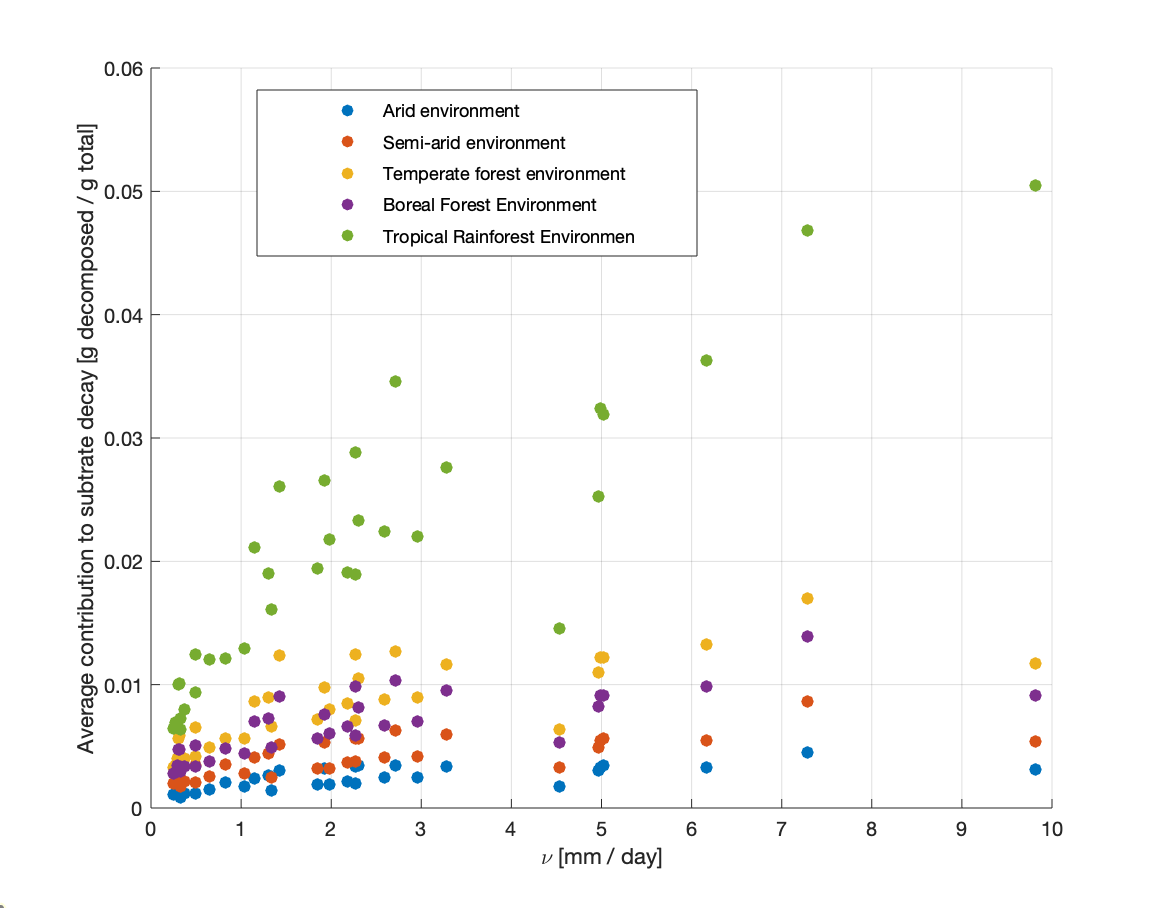
\includegraphics[width=0.7\linewidth]{avg_contr_nu_environment.png}
%	\caption[Fig 1.]{Example optimized flight plan, ran with drone fleet size of 5, starting configuration 1, 5 allowed movements, and $\gamma$ = 2}
%	\label{Fig 1.}
%\end{figure*}

\subsection{Decomposition kinetics}
Moore et al. (2015), Edelstein (1983), Moorhead et al. (2006), Parnas (1974), and Schimel et al. (2003) describe the decomposition of a certain substrate by a microbial decomposer as a function of the substrate's concentration by the Michaelis–Menton equation \cite{Moore2015, Edelstein1983, Moorhead2006, Parnas1975, Schimel2003}. Schimel et al. (2003) and Moorhead et al. (2006) assert that decomposition levels off at a maximum rate proportional to the concentration of enzymes acting on it \cite{Schimel2003, Moorhead2006}. The decompostion of carbon in a substrate is described by the following equation.

\begin{equation} \label{eq:3}
\frac{dC}{dt} = \frac{KBC}{K_{e}+C}
\end{equation}
We make the assumption that the enzyme concentration is proportional to the concentration of biomass in our system represented by $r$ multiplied by two environmental limiting factors in $K=rS_{M}S_{T}$ \cite{Schimel2003}. Moorhead (1990) uses these limiting factors to multiply the rates of carbon uptake from microorganisms, although the model used a simpler first order, linear equation \cite{Moorhead2006}. Here we use it in a similar way in limiting our maximum decay rate. The factors, $S_{M}$ and $S_{T}$ are computed by the following equations:
\begin{equation}
S_{M}=\alpha_{2} - \lambda \log_{10}(-\psi)
\end{equation}
\begin{equation}
\log_{10}(S_T) = \frac{T-25}{10}\log_{10}(Q)
\end{equation}
\pagebreak
\section{Model Formulation}


\subsection{Growth Model}
In the review of various fungal growth models described in Lin et al. (2016), a specific method of modeling branching and hyphal death was found to match experimental observations in the widest variety of settings. Based on these results, for $\sigma$ and $d$ in (\ref{eq:1}) and (\ref{eq:2}) we will choose to implement the following relationships, comprising dichotomous branching, tip-hypha anastomosis, and hyphal death (or YHD). 
\begin{equation} 
\sigma = \alpha_{1}*n - \mu n \rho
\end{equation}

\begin{equation}
d = \gamma_{1}\rho
\end{equation}

Enzymes conducting decomposition make up a fraction of the total biomass, and the total biomass changes according to the growth rate. The total biomass $B$ defined in (\ref{eq:8}) multiplies by maximum rate of the Michaelis-Menion equation (\ref{eq:3}) to couple growth rate with decomposition rate. 

\begin{equation} \label {eq:8}
B = \int_{all x}\rho dx
\end{equation}

The rate of decomposition of carbon will then be dynamically effected by the growth of the fungus contrary to the typical assumption of a static $B$ as described by Schimel et al. (2003) \cite{Schimel2003}. Our formulation of $K$ which accounts for the proportion of biomass in the fungal growth containing the necessary enzyme for the carbon decomposition will change to account for this. 
\begin{equation} \label {eq}
K = r*S_{M}*S_{T}*0.04*G
\end{equation}
Where $r$ is a dimensionless parameter representing the relative abundance of one enzyme out of the total enzyme biomass of that specific fungus. The multiplication by $0.02$ is a generalization that for any given species of fungus, 2\% of the biomass will be relevant enzymes \cite{Moorhead2006}. $G$ is an empirically derived rate constant relating the mass of relevant enzymes to the maximum rate of the decomposition.

TALK ABOUT ENZYMES FROM DATA IN MAYNARD

Limited carbon availability will also impact a fungi's growth rate. To account for this, we include a term multiplying $\nu$ that can be interpreted as the available carbon for the fungi to consume for growth. The first equation in the growth model then becomes
\begin{equation} \label{eq:10}
\frac{\partial \rho}{\partial t} = (1-LCI)*(10^{9})*C*n*\nu - d
\end{equation}
Where $LCI$ is the lignocellulose index\footnote{The lignocellulose index describes the ratio of non-hydrolysable lignin to hydrolysable holocellulose in litter} of a certain material and $(1-LCI)$ is then the proportion of the substrate carbon stored in holocellulose. Multiplying by $(1*10^{9}$ is approximation to convert grams of carbon to hyphae length in mm. [citation needed for g to mm] An investigation of the effects of including the carbon term in the growth model are addressed in a later section. \\

So our coupled growth and decomposition models can be summarized by equations (\ref{eq:2}), (\ref{eq:3}), (\ref{eq:8}), and (\ref{eq:10}).

\subsection{Estimating $\nu$ For Various Environments}

When considering a sampling of decomposition rates in various environment types, we must determine how to estimate temperate and water potentials that ground fungi would experience. In the case of determining $\nu$, this requires finding projected temperature and water potential.

Amongst existing biome classification models, Whitaker's scheme \cite{Whittaker1970} is perhaps the simplest, being particularly trait-based. Whitaker's scheme provides a layout of biomes based on mean annual temperature and mean annual precipitation. However, modern classification of biomes has drifted away from using these traits as definitive biome identifiers \cite{Mucina2018}. These traits alone do not define all features of concern to fungal growth, such as soil composition for example. In addition, by Whitaker's scheme, we find that a given biome can have a wide range of average annual temperatures (such as arid desserts ranging from about -10 to 30 $^{\circ}C$) \cite{Whittaker1970}. Thus, we can sample a range of temperature and moisture values to output various $\nu$ and then select certain regions to profile in order to gauge potential environments where fungi can decompose and interact.
%We will sample within the temperature range of Whitaker's scheme: $-15^{\circ}$ to $30^{\circ}$ C of mean annual temperature.

The following are the specific environments selected to represent various biomes:

\end{multicols}

\begin{savenotes}
	\begin{table}[H]
		\begin{center}
			\begin{tabular}{|c c|} 
				\hline
				Biome & Specific Environment Selected \\ [0.5ex] 
				\hline\hline
				Dessert (Arid) & Sonoran Desert, USA \\ 
				\hline
				Grasslands/shrublands & (Semi-Arid), central Argentina\\
				\hline
				Temperate Forest & Sal Forests, central Himalayas\\
				\hline
				Boreal Forest (Arboreal) & Pine Forests, central Himalayas\\
				\hline
				Tropical Rain Forest & Tropical Forests, Barro Colorado Island, Panama \\
				\hline
			\end{tabular}
		\end{center}
	\end{table}
\end{savenotes}

Although water potentials can be approximated based on predictive models, the measure is best found experimentally from soil samples \cite{Abkenar2019}. Ranges for moisture potential of these environments have been found experimentally from a variety of studies is shown in the following table************. Note that single water potentials and temperatures are selected for sampling, as we are aiming to compare discrete environmental conditions rather than create a complete span of environmental conditions. The following are the selected values of average annual temperatures and water potential for these biomes. If ranges are given, the average of the ranges or seasonal values is the selected value. For full ranges and data sources, see appendix TABLE ???.

%% ACTUAL TABLE
\begin{table}[H]
	\begin{center}
		\begin{tabular}{|c c c|} 
			\hline
			Biome/ Environment & Temperature [$^{\circ}C$] & Water Potential [MPA]\\ [0.5ex] 
			\hline\hline
			Dessert (Arid) & 15 & -4.5 \\ 
			\hline
			Grasslands/shrublands (Semi-Arid) &15.3 & -3.2\\
			\hline
			Temperate Forest & 12.49 & -1.09 \\
			\hline
			Boreal Forest (Arboreal)& 12.49 &  -1.51 \\
			\hline
			Tropical Rain Forest & 27.5 & -0.79 \\
			\hline
		\end{tabular}
	\end{center}
\end{table}


Given these estimates, we can have a probable example combination of temperature and moisture potential in various environments. Note that these are not wholly representative configurations, but rather examples to provide insight into how fungal species with specific traits may respond in discrete and distinct conditions likely to exist. 

We can then find $\nu$ using experimental data from Maynard et al 2019. **** (talk about continuous data technique thingy in the extra methods info sheet)

\begin{multicols}{2}
	
\subsection{Other Responses to Temperature and Water Potential}

Our growth model takes into account temperature (T) and water potential ($\psi$) in two more parameters: the soil temperature coefficient ($S_T$) and the soil temperature coefficient ($S_M$). Moorhead et al. (1991) provides a simple relationship between $S_T$ and T using the rate of increase (Q):
\begin{equation}
\log_{10}(S_T) = \frac{T-25}{10}\log_{10}(Q)
\end{equation}
Although this equation does not take into account specific fungal response to temperature change, more recent evidence supports that this relationship is not direct, with most of the direct impact coming from moisture \cite{Petraglia2018}. As the ratio of rates of decomposition given a temperature change, Q as a parameter should represent the effective output of various mechanisms influenced by temperature rather than focusing on specific mechanisms. However, for the sake of simplicity, Q has been set standard constant to a value of 2.5 \cite{Moorhead1991}.

Water potential also relates to a constant, $S_M$, in a simple equation described in Moorhead et al. (1991) using $\alpha_2$ and $\lambda$:
\begin{equation}
S_M = \alpha_2 -\lambda \log_{10}(-\psi)
\end{equation}

These two parameters help calculate the maximum growth rate by the relationship:
\begin{equation}
\beta = S_T S_M r
\end{equation}
where r is the enzyme biomass ratio.

\subsection{Assumptions}
\subsubsection{Growth}
\begin{itemize}
	%\item Growth occurs in a 1-dimensional space *we should mention this in the formulation
	\item Neglecting effects from direct interactions between fungi
	\item Neglecting effects from N limitation
	\item Litter is not added to or removed from the carbon pool by forces external of the fungi
	\item LCI is xxx and remains constant over time
	\item Dynamics regarding the rate of nutrient absorption and transport of metabolites within the
	mycelium are ignored or simplified *more specific
	\item Ignoring other growth traits: LIST
	%\item Substrate use efficiency (SUE) is 1 *should be in the model formulation
	\item Hyphal death rate $\gamma_{1}$ remains constant regardless of environmental fluctuations
	\item 100\% of living hyphal tips are active
	\item No biomass created by a fungus will be geometrically isolated from the substrate
	\item Neglecting effects due to spacial limitations
	%\item decomposition coefficients are representative of those families of enzymes
\end{itemize}
\subsubsection{Decomposition Kinetics}
\begin{itemize}
	\item Neglecting effects due to enzymes not included in the model
	\item Production of enzymes increases proportionally with biomass
	\item For any species of fungus, 2\% of the biomass will be relevant enzymes
	\item Relative proportions of enzymes will stay constant regardless of environmental fluctuations
	\item Neglecting effects on decomposition rate due to changing metabolic rate of the fungi
\end{itemize}
\subsubsection{Temperature/Moisture effects}
\begin{itemize}
	\item Turgor is a function of water potential
	\item Fungal decomposition occurs in surface soil (0-30 cm)
	\item Experimental data for water potentials in specific biomes/environments are representative of the conditions of those environments
	\item Rate of increase of temperature $Q$ remains constant regardless of environmental fluctuations
\end{itemize}

\section*{Parameter selection and representative result}
To select realistic values for the parameters, we created a representative run of the coupled growth and decomposition model, consulting the literature to find parameter values. An overview of the parameter selection for this representative run can be seen in (parameter table), however several parameters are worth some discussion. 
\subsection*{Growth model parameters}
The effect of two main parameters were studied for their effect on the growth model's result: the branching rate and the hyphal death rate. These parameters were not agreed upon in the literature so their effect on the model output was evaluated and they were selected from a pool of possible values based on the most likely realistic output. Most results of the growth model were comprised of traveling wave solutions, converging to a uniform distribution in both space and time. This can be thought of a the maximum growth of the fungus into it's total space. The branching rate ($\alpha_{1}$) was found to increase the hyphal density in the end behavior of the solution, with the ending density increasing as $\alpha_{1}$ increases. The hyphal death rate ($\gamma_{1}$) was found to increase the oscillations in time and thus larger $\gamma_{1}$ values would increase the oscillations and the time to reach a given end-behavior. Many of the papers discussing the values of these parameters [Edelstein 1982] [Lin 2016] [Schnepf 2007] [Du 2019] are concerned more with short term dynamics in perfectly ideal conditions. The purposes of this paper is the assess the long term decomposition rates under different conditions, so parameters that can predict long-term behavior, comparable to long term decomposition dynamics described in [Moorhead 2000] [Moorhead 2006] [Moorhead 1991] were selected.

\end{multicols}
\begin{center}
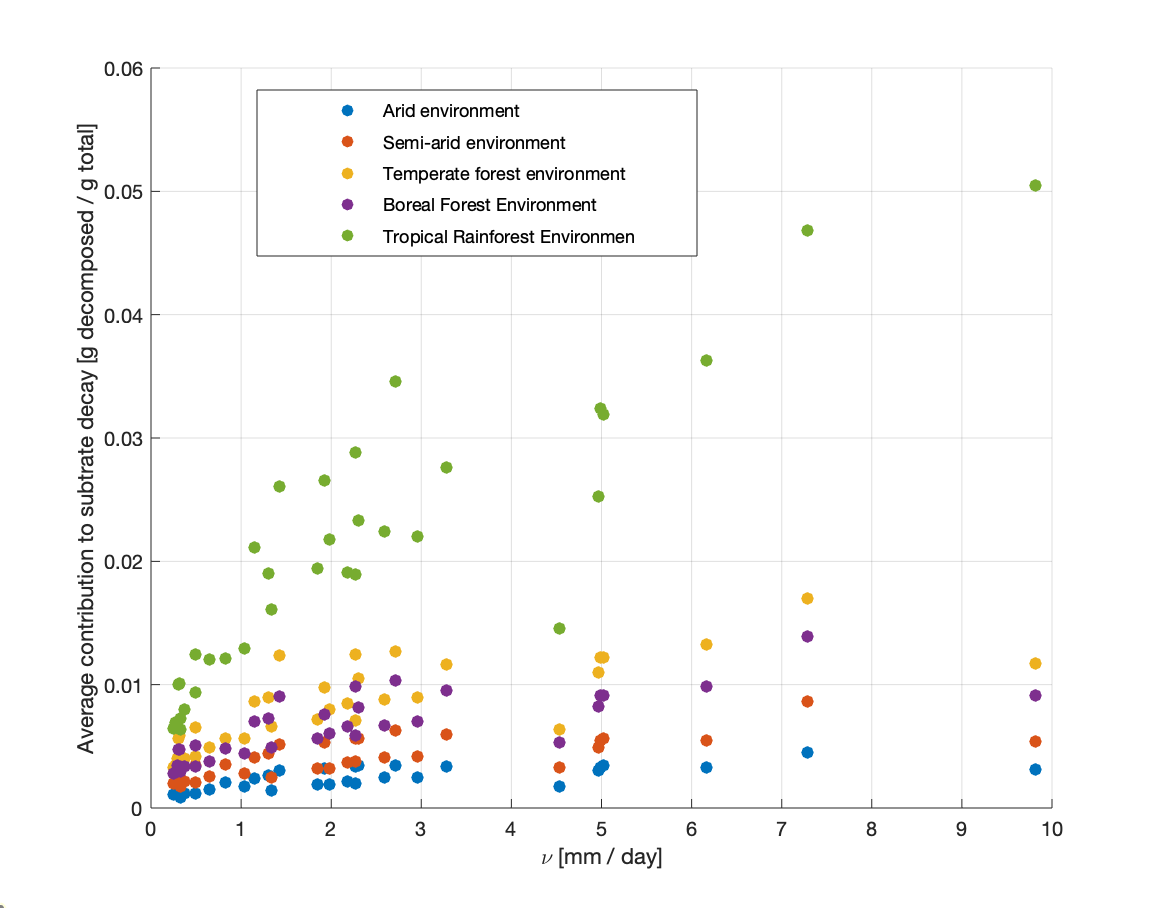
\includegraphics[width=\linewidth]{avg_contr_nu_environment.png}
\captionof{figure}{Figure caption}
\label{Fig 2.}
\end{center}
\begin{multicols}{2}

\subsection*{Decomposition parameters}
The value for $G$ is interpreted as a rate constant, relating a concentration of relative enzymes to the maximum rate of carbon decomposition. formulation for $S_{M}$ and $S_{T}$ come from [Moorhead 1991] and in said model, a simpler equation is used for the reaction dynamics for decomposition of carbon. Because of this, we cannot use the same rate constant and must base this parameter of agreement with other models or experimental data. The most important aspect we examined for the section of $G$ was the timescale of decomposition to be comparable with that of [Lustenhouwer 2019].
\subsection*{Representative results}
As a representative result of the coupled growth and decomposition model, the two were run using the parameters summarized in (parameter table). In the growth model, $\rho$ was found to exibit travelling wave dispersion throughout space, as similarly shown in [Mimura 2000] and [Edelstein 1982]. Due to the simulation only running for a timespan of 3 years, the decrease in carbon over time looks fairly linear, with slight fluctuations likely due to the fluctuating fungal biomass densities over time. The first initial runs were done without the coupling term in the growth equations, so the growth model was assuming an abundance of nutrients and not affected by the decreasing concentration of carbon. Depending on the timescale being simulated, that could be a perfectly valid assumption, as short time scales tended to show little overall decrease in the concentration of holocellulose carbon. However the differences seen in including the nutrient availability term in the growth equations become more apparent as longer time scales are considered. The effects of this can be seen in our results. The overall biomass was also mostly unaffected other than replacing decaying oscillations towards a steady state with a somewhat constantly increasing biomass overtime with a decaying slope. Overall, including the nutrient availability term in the growth equation captures more of the fundamental interaction that this paper is concerned with (that of decomposing wood and ground litter rather than free-growing fungi), so it was included in further analysis. 


\section*{Fungal species interaction}
Due to the complex mechanisms of direct interaction between fungi, we chose to focus not on the direct interactions between the fungi in their consumption of the substraight, but on the interactions caused by differing rates of decomposition among different enzymes in varying environmental conditions and how the relative amounts of different bacteria in a fungi species will impact its competition. This was formulated in the model by taking the weighted sum of all contributions to the decomposition rate from any one of four enzymes in a given fungi species, represented in the following equation
\begin{equation} \label{eq}
\frac{dC_{1}}{dt} = c_{1,a}\frac{de_{1,a}}{dt} + c_{1,b}\frac{de_{1,d}}{dt} + c_{1,c}\frac{de_{1,c}}{dt} + c_{1,d}\frac{de_{1,d}}{dt}
\end{equation}
Where $c_{1,a}$ is a enzyme breakdown efficiency coefficient for the fungal species $1$ and enzyme $a$. Here the rate $\frac{dC_{1}}{dt}$ is representative of the rate of decay of the substrate by the fungi species $1$. The total decomposition rate is then given by the sum of all rates over the various species of fungi.
\begin{equation} \label{eq}
\frac{dC_{tot}}{dt} = \sum_{i=1}^{n}\frac{dC_{i}}{dt}
\end{equation}
Where $n$ is the total number of fungi being simulated. 


\begin{ColumnFigure}
	\centering
	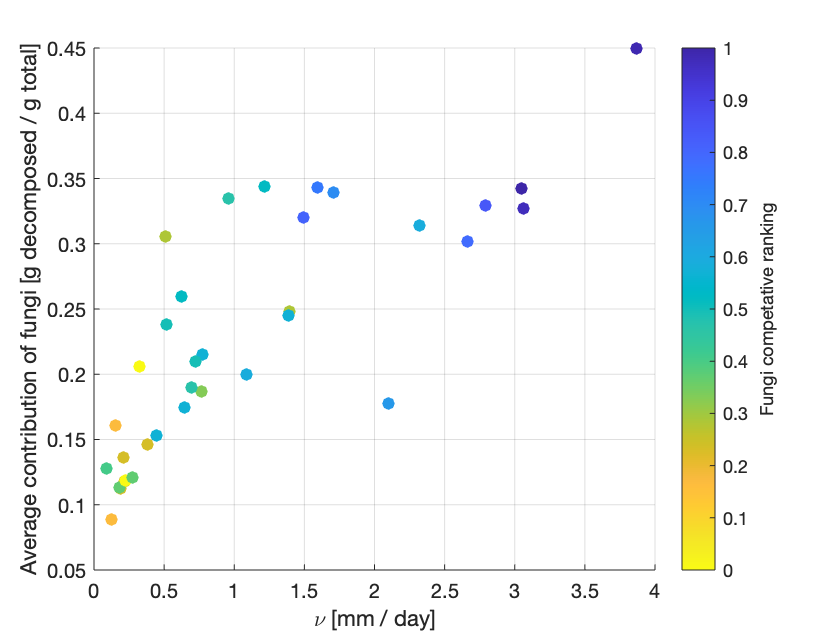
\includegraphics[width=\linewidth]{avg_contr_nu_competative_rankings.png}
	\captionof{figure}{my caption of the figure}
\end{ColumnFigure}


\subsection{Environmental Influence on Hyphal Tip Extension}

\subsection{Decomposition Kinetics}

\subsection{Enzyme Implementation}

\subsection{Moisture}

\section{Pre-planning intro}

The Five Core Tenants:
1. growth/Decomposition continuous model
- general explanation of the structure of fungi: hyphal extension rate, branching, tips, death, etc.
- proportion of enzymes relative to the phases correlates with the speed of decomposition and effectiveness in a certain phase
- substrate talk - LCI, lignin inhibition of holocellulose, common substrate compositions, how soil is different
- phases talk
- reasoning behind choosing a continuous model

2. interactions between different fungi with differing characteristics
- competitive interactions *
- synergy under richness and fluctuating temperatures *
- the more differing the characteristics of the fungi, the more likely they are to compete
- the competitive ranking *

3. sensitivity to environmental fluctuations
- slower-growth stress tolerant fungi vs fast growth more niche temp/moisture fungi determining which of these two wins out depends on how much the environment is fluctuating and what subset of fungi are present *
- fluctuating temperatures promotes growth
- moisture talk *
- biome talk

4. biodiversity's impact on systems overall efficiency
- richness promotes growth
- competition promotes efficiency *
- dominant species that 'wipe out' the community generally harm? *

5. effect on the carbon cycle
- fungi/bacteria are the only life forms which can break down lignin and efficiency break down holocellulose litter — these poysaccarides make up a huge portion of the total ground litter biomass in the earth's forests

Biodiversity's impact on the system's overall efficiency:
- the greater range you have of moisture/temperature niche widths, the more tolerant your fungal community will be overall to growing in any particular environmental because at least some constituents of the community will be close to idealized in that environment.
- competition rank correlates heavily with hyphal extension rate — fungal communities with species who are highly competitive will go one of two ways: 1. the environmental conditions are ideal for the smaller niches of the highly competitive isolates, and so those isolates will dominate out over the other ones 2. the environmental conditions are not ideal for the highly competitive isolates, so the slower but more robust isolates will win out

we have a spearman correlation coefficient relating production of each enzyme with decomposition rate — enzymes primarily involved with breaking down lignin (acid phosphatase) are strongly correlated with decreased decomposition rate.

Strong correlation that increase production of acid phospatase results in decreased competitive rank, which makes sense because on average slower-growing fungi are less competitive than faster growing ones. Competitive rank has a 0.6 spearman correlation coefficient with growth performance

Assumption: enzymes treatment of the different portions of holocellulose are the same 

Implementation: each enzyme has its production rate from the data, multiply the parameter by that production rate and sum them all together to get dC/dt

Recapitulating previous literature


Prediction:
The slower stress tolerant fungi will have a share of enzymes that indicate their slow decomposition rate, but a moisture and temperature width that indicate their stress tolerance to environmental fluctuations. 

The faster fungi will have a share of enzymes that indicate their fast decomposition rate, but a moisture and temperature width that indicates their lack of stress tolerance to environmental fluctuations.

\section{Model formulation}
Maynard et. al took data on the productive rates of 8 different enzymes (5 hydrolytic and 3 oxidative to cover the spectrum of the cellulose-degradation process) and used a standard clustering approach to determine 4 representative enzymes of the entire set: cellobiohydrolase, acid phosphatase, peroxidase and phenoloxidase. The data for production of these enzymes comes from their open-source github. 

We're making the assumption that the production of each enzyme is  equivalent to the amount of the enzyme present in the fungus. We took the production data and normalized it to z-score values. Each z-score was turned into a portion of that enzyme with $e_x$ = (z-min)/(max-min) and then we divided each portion by the sum of all enzyme portions for each enzyme $(e_x)/(e_1+e_2+e_3+e_4)$. This gives us a representation of the proportion of each enzyme relative to other enzymes. We made the assumption thatt the total mass of those four enzymes for each fungus is the same, and the fraction of enzyme mass from total mass.

We made the assumption that the enzymes are not changing over time due to C/N changes or environmental fluctuations

The time scale for our model is following the experimental results from (paper cited by question) which indicates x\% log decomposition after 3 years and y\% decomposition of logs after 5 years for a wide sampling of fungus

\subsection{Assumptions}

\begin{itemize}
	\item Growth
	\begin{itemize}
		\item unlimited available resources (ground litter and woody fibers)
		\item neglecting effects from direct interactions between fungi
		\item PROBLEM: neglecting synergistic effects on growth/metabolic efficiency
		\item non-exhaustive substrates
		\item not considering N addition by anthropogenic nitrogen deposition
		\item LCI < 0.7 at all times because we're focusing on wood fibers and we don't want lignin block holocellulose decay in bad ways. but we could use the formula
		\item LCI is not changing over time anastomosis, the formation of reconnections. 
		\item dynamics regarding the rate of nutrient absorption and transport of metabolites within the
		mycelium are ignored or simplified
		\item growth dynamics incurred by the formation of concentric density rings are not considered <-- this doesn't need to exist because we're considering growth in a 1D tube
		\item only considering one configuration of growth traits out of many possible options, that configuration being: tip-hypha anasmotosis, dichotomous branching, and hyphal death
		\item decomposition coefficients are representative of those families of enzymes
	\end{itemize}
	\item Decomposition Kinetics
	\begin{itemize}
		\item[--] Elements can be stacked in any configuration without structural limitations
	\end{itemize}
	\item Temperature/Moisture effects
	\begin{itemize}
		\item[--] experimental data for water potentials in specific biomes/environments are representative of the conditions of those environments 
	\end{itemize}
\end{itemize}


\subsection{Cost Function}
I've copied the ten diff eqs from Numerical Prediction Model for Fungal Growth Coupled with Hygrothermal Transfer in Building Materials here:

hygrothermal equations:

\begin{equation}
\frac{dH}{dT}\cdot\frac{\partial T}{\partial t}=\nabla\cdot(\lambda\nabla T)+h_v\nabla\cdot(\delta_{p}\nabla(\phi p_{sat}))
\end{equation}

\begin{equation}
\frac{dw}{d\phi}\cdot\frac{\partial \phi}{\partial t}=\nabla\cdot(D_{\phi}\nabla\phi+\delta_{p}\nabla(\phi p_{sat})
\end{equation}

Chapter 15 Mathematical Modeling of Fungal Growth

\begin{equation}
\frac{\delta\rho}{\delta t}=nv-d(\rho)
\end{equation}

\begin{equation}
\frac{\delta n}{\delta t}=\frac{\delta nv}{\delta x}+\sigma(\rho, n)
\end{equation}


Where $P$ represents the total medpacks delivered, $\sum{t}$ is an estimate of the time for all the flights to occur, and $S$ represents the space left after packing all the drones (computed via the packing algorithm). Also, $C$ is our cost function output, the cost. The factor of $100000$ dividing $S$ is there to adjust the units of $S$ (it being on the order of $10^5$ while $\frac{P}{\sum{t}}$ is on the order of $10^0$) The time estimates are computed via the basic kinematic equation assuming constant speed, $\sum{t}=\sum{\frac{d}{v_d}}$ summed over all drone flights in the given plan. Here $d$ is distance traveled in a specified flight and $v_d$ is the max speed of the drone flying. This estimate of the time taken for a flight is assuming the drone is flying at max speed the whole way, and assuming equality of the time taken to fly to the hospital, and the time to fly back. The assumption of perfectly sequential ordering of the flights allows us to sum the times of individual flights to get the total time.

\section{Results and Analysis}
% TODO: \usepackage{graphicx} required
%\begin{figure*}
%	\centering
%	\includegraphics[width=0.7\linewidth]{}
%	\caption[Fig 1.]{caption 1}
%	\label{Fig 1.}
%\end{figure*}

\subsection{Model output}
\lipsum[6]

\subsection{Parameter sensitivity}
\lipsum[7]

% TODO: \usepackage{graphicx} required
%\begin{figure}
%	\centering
%	\includegraphics[width=1.1\linewidth]{}
%	\caption[Fig 2]{caption 2}
%	\label{Fig 3}
%\end{figure}

% TODO: \usepackage{graphicx} required
%\begin{figure}
%	\centering
%	\includegraphics[width=0.9\linewidth]{}
%	\caption[Fig 3]{caption 3}
%	\label{Fig 4}
%\end{figure}


\subsection{Limitations/ Further Work}
\lipsum[8]

In all models, the terms for $\nu$, $\sigma$ are taken to be constants given from experimental data. [citations]. Lin et al. (2016) takes a different approach in reviewing previous literature to apply a model that closely matches experimental data, which we will take advantage of for our model.  

\end{multicols}
\printbibliography
\end{document}